\documentclass[11pt]{article}
\usepackage[a4paper,margin=1in]{geometry}
\usepackage{graphicx}
\graphicspath{{rfigs/}}
\usepackage{enumitem}
\usepackage{xcolor}
\usepackage{mdframed}
\setlength{\parindent}{0pt}  % No indentation
\setlength{\parskip}{10pt}   % Space between paragraphs
% Toggle this to enable/disable highlights
\newif\ifhighlight
\highlighttrue % Uncomment to enable highlighting
% \highlightfalse % Uncomment to disable highlighting
\newcommand{\hl}[1]{\ifhighlight\textcolor{blue}{#1}\else#1\fi}

\newmdenv[
  topline=false,
  bottomline=false,
  skipabove=\topsep,
  skipbelow=\topsep
]{siderules}
\begin{document}

\section*{Response to Reviewer 3}

\begin{siderules}
\textit{This manuscript investigates the fringe pattern around a wet beet slice, a common phenomenon observed in one’s kitchen. The authors combine systematic experiments (measuring the evolving shape of the liquid film) and simulations to rationalize this phenomenon. Their results show that the fringe pattern is caused by the dimple formation on the liquid surface, as the contact line rises on the beet surface, unifying existing hypotheses. Overall, the paper is a worthy contribution to Physical Review Fluids, as it addresses a relatable problem and explains with sound fluid mechanics principles. I have some minor questions and comments about the manuscript that I list below.
}
\end{siderules}

\bigskip
\begin{siderules}
\textbf{Comment 1:} \textit{The authors refer to Fig. 4(c) on line 117, but I don’t see Fig. 4(c) in the manuscript. I assume this is a typo.}
\end{siderules}

\textbf{Response:} We thank the reviewer for pointing out the typo. 
\hl{We fixed the figure labels in Fig.~4.}

\bigskip
\begin{siderules}
\textbf{Comment 2:} \textit{The central result of the manuscript is that the porous nature of the beet or the Marangoni effects are not the necessary physical ingredients that cause the fringe formation, disapproving and unifying the previous hypotheses. Instead, the authors show that the wetting properties (small $\theta$s) and the thickness of the liquid film are what allow the dimples to form and even persist for the fringe pattern to be visible. While the authors’ claim is quite convincing, it would make the manuscript even stronger if the authors can include similar experimental observations with different solid materials other than beet. Have the authors tried recreating the fringe patterns using different surfaces (that are indeed not porous)? If the authors have not been able to recreate them, maybe it speaks to the fact that the wetting conditions that are necessary to create a dimple are very specific and not easy to achieve. Can authors elaborate on this? Namely, either include experimental observations on non-porous materials or explain why such observations are difficult to achieve. Overall, proving the generality of the phenomenon in question would strengthen the current manuscript quite a bit.
}
\end{siderules}

\textbf{Response:} We thank the reviewer for bringing the idea of testing different solid materials to our attention. We did test a few other materials, porous (tissue, foam) or nonporous (coin, rubber). We saw the fringe pattern around all of them, as long as the liquid film is thin enough. These tests led us to think that being porous was not necessary. 

In Fig.~\ref{fig:coin-fork}, we attach a picture, where coins and a fork induced fringes in a thin film of beet juice (picture courtesy Zak Kujala @ UMN). 
We got this picture after we presented this work at APS DFD 2024. 
Zak reached out to us regarding this “different materials” question. 
This picture perfectly illustrates that this phenomenon is not specific to beet. Nonporous solid materials, like coins and forks, can also induce the fringe pattern. 

\hl{
In the revised manuscript, we included a picture in Fig.~1 (again from Zak), where a coin (hydrophilic) and a PDMS cylinder (hydrophobic) are put in a thin film of beet juice, to demonstrate that porousness is not a necessary condition to induce the fringe pattern.
}

\begin{figure}[ht]
    \centering
    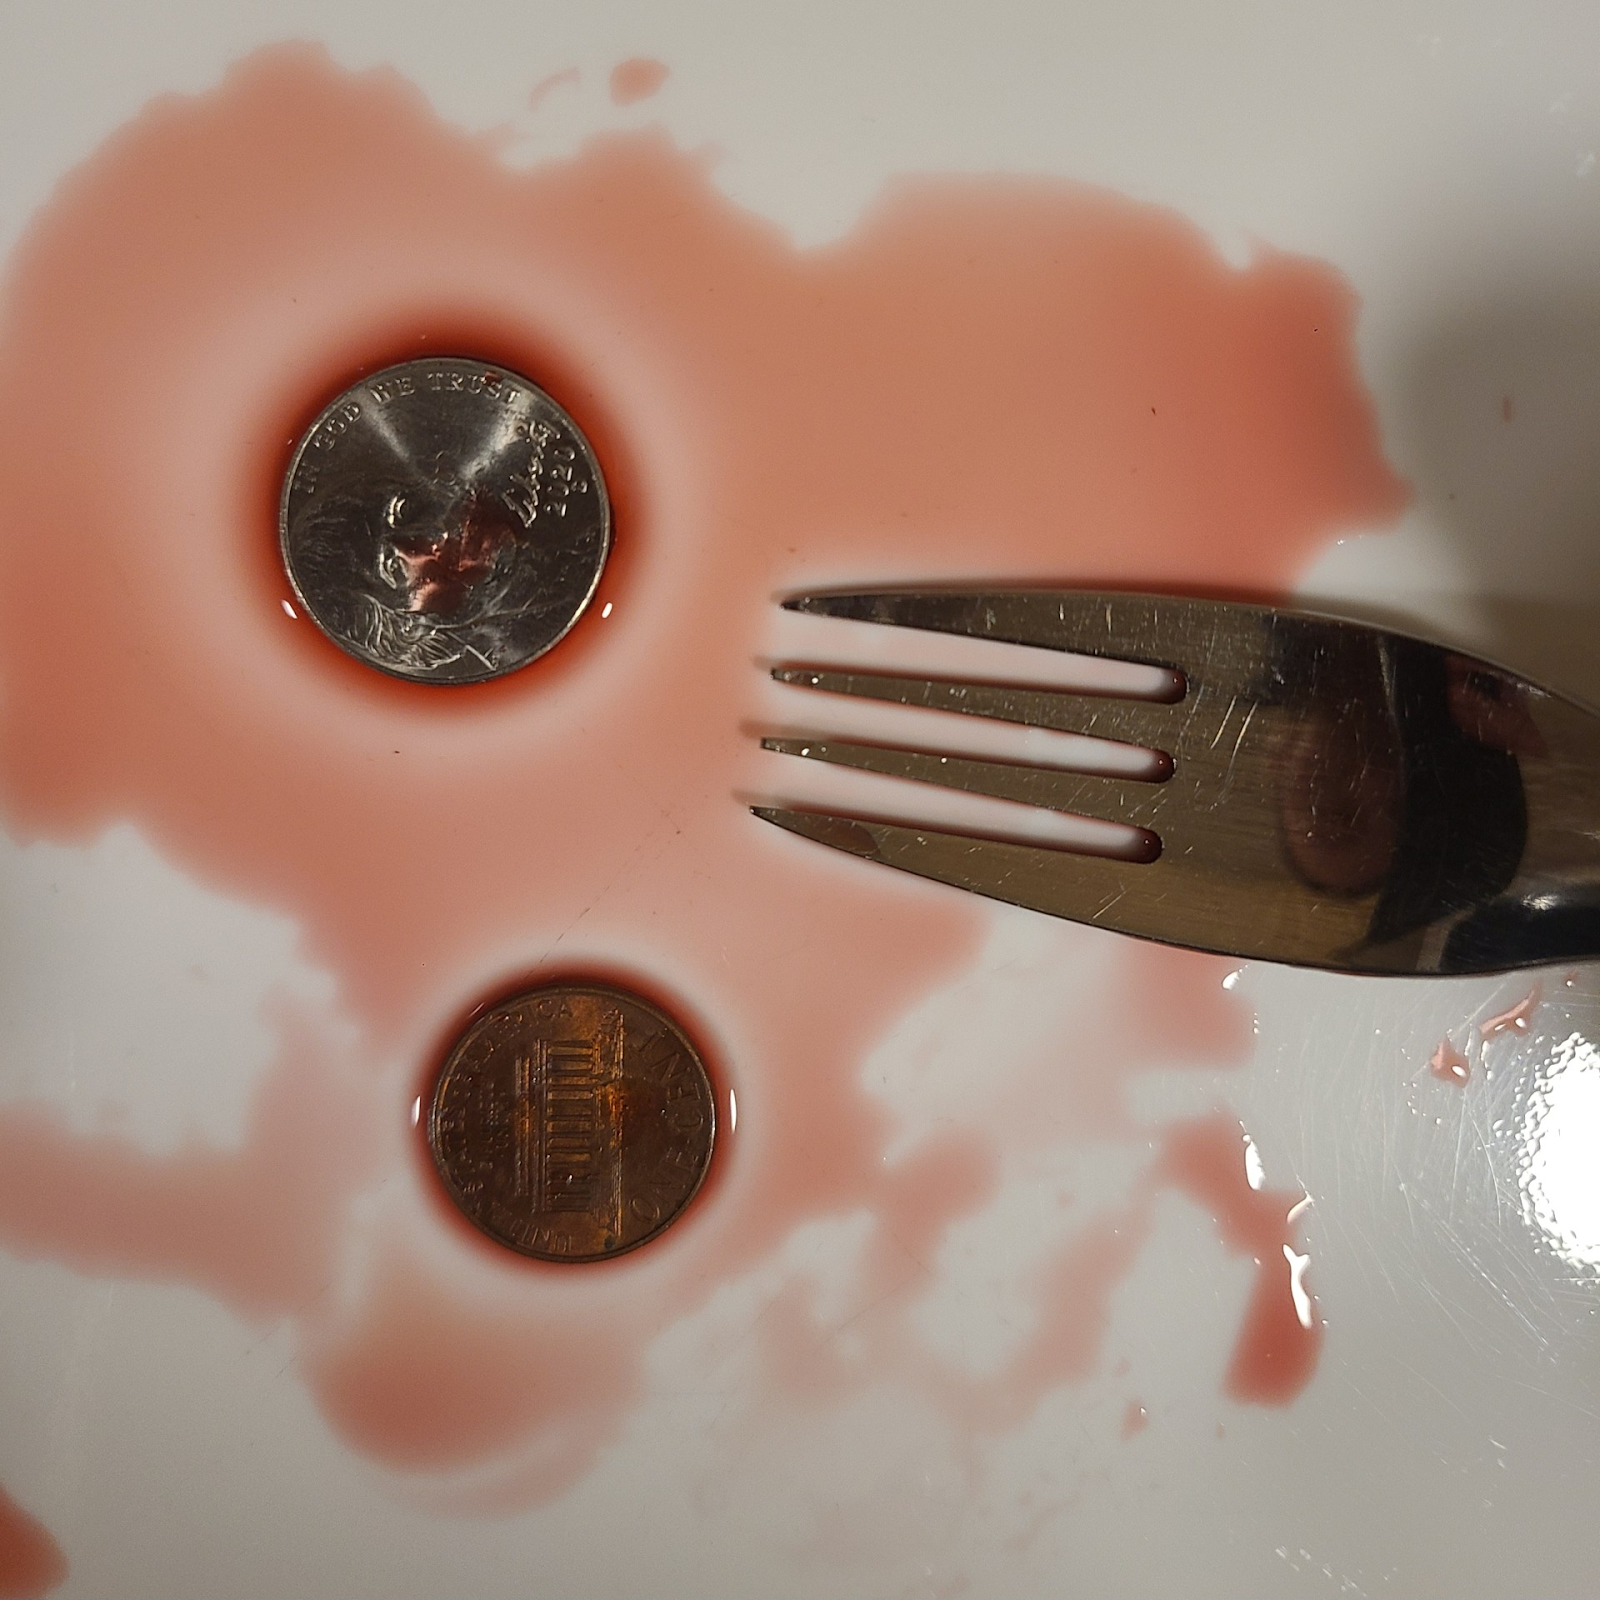
\includegraphics[width=0.5\linewidth]{coin_fork.png}
    \caption{Fringe patterns induced by coins and a fork.}
    \label{fig:coin-fork}
\end{figure}

\bigskip
\begin{siderules}
\textbf{Comment 3:} \textit{
I have questions regarding the governing equations (3)-(4) on page 9. 
Unless I am mistaken, Eq. (3) is valid only when your flow is primarily uni-directional, which would be the case if the interfacial deformations are relatively “small” and, hence, are suitable for lubrication theory. 
However, Eq. (4) uses a full curvature term that does not assume small slope. 
To me, this looks inconsistent. 
Can the authors explain this? 
Along the same lines, the authors should explicitly include all the model assumptions that have gone into deriving equations (3)-(4). 
Also, if you simplify Eq. (5) so that the curvature term only contains $h''$, how does this affect the simulation results? 
I am assuming that it should not affect them very much, but I would appreciate the authors’ insight.}
\end{siderules}

\textbf{Response:} We thank the reviewer for the insightful question. Indeed, the lubrication theory assumes a thin film and a unidirectional flow in $x$. 
The thin film assumption, in turn, leads to $p=\sigma h''$. Including the prefactor of $h''$ seems unnecessary. 
Here, we run the simulation with and without the prefactor for the same initial conditions ($h_0=0.3$ mm). The results are shown in Fig.~\ref{fig:prefactor}. 
We also show the experimental data with a similar film length and initial thickness.

\begin{figure}[ht]
    \centering
    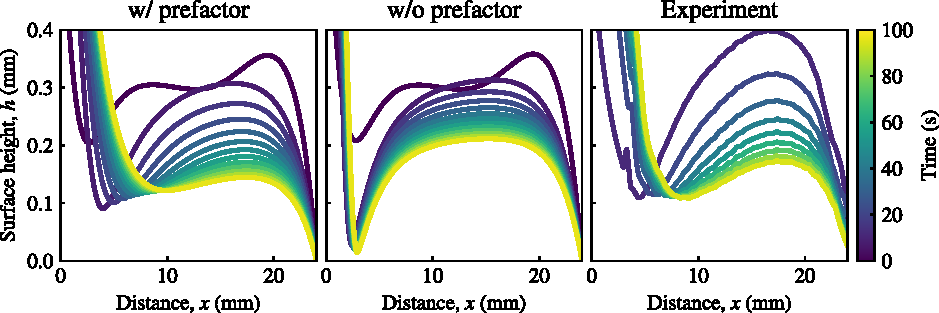
\includegraphics[width=0.9\linewidth]{Figures/prefactor.pdf}
    \caption{Simulated surface evolutions with (left) and without (right) the prefactor of $h''$.}
    \label{fig:prefactor}
\end{figure}

We found that, without the prefactor, the dimple relaxation process becomes extremely slow. 
This makes sense, as the prefactor amplifies the negative pressure in the meniscus, sucking more fluid to the meniscus. 
The simulation with the prefactor also agrees with the experimental observation better. 

\hl{We added one sentence like ``Although it seems inconsistent to include the prefactor $[1+(\partial h/\partial x)^2]^{-3/2}$ in Eq.~(2) with a thin film approximation, we find that this prefactor in simulations better predicts experimental surface profiles (see Fig.~\ref{fig:prefactor}).''. Also, we included Fig.~\ref{fig:prefactor} to Appendix D in the revised manuscript.}

\bigskip
\begin{siderules}
\textbf{Comment 4:} \textit{I do not find the collapse of the dimple time data (inset of Fig. 5(d)) to be as convincing, especially because the collapsed plot is very small and difficult to see. Can the authors include the larger plot so that the readers can judge if rescaling the dimple time data does in fact work? Also, what are the associated errors in measuring the film height and the dimple time from the experiments? (I do not see any error bars on the measurements, perhaps because the errors are rather minimal. I would like an explanation either way.)}
\end{siderules}

\textbf{Response:} We thank the reviewer for pointing out the issue with the collapse plot. 
In Fig.~\ref{fig:collapse}, we provide larger $t_\mathrm{dimple}$ plot, raw and rescaled. 
%Comparing Figs.~\ref{fig:collapse}(a) and \ref{fig:collapse}(b), we can see that the two curves for 60\% and 80\% glycerol-water mixtures collapse, but the beet juice curve is still isolated, suggesting that the rescaling correctly accounts for the effect of viscosity, but not for surface tension. 

% \begin{figure}
%     \centering
%     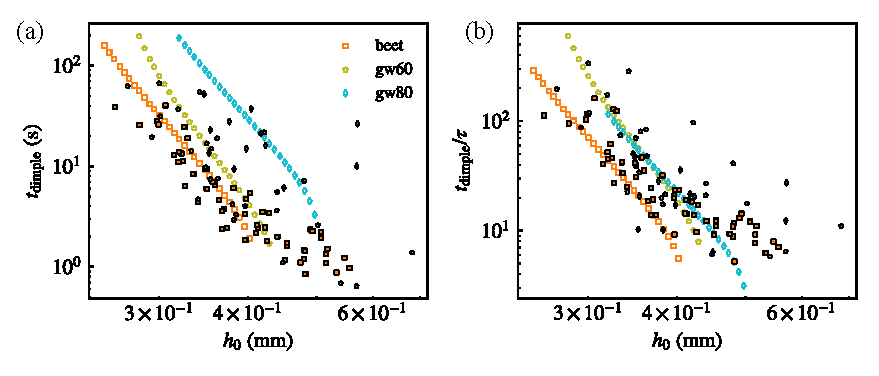
\includegraphics[width=0.9\linewidth]{collapse}
%     \caption{$t_\mathrm{dimple}$ (a) and rescaled $t_\mathrm{dimple}$ (b) vs. $h_0$.}
%     \label{fig:collapse}
% \end{figure}

\hl{
In the revised manuscript, we revised the scaling analysis on how $t_\mathrm{dimple}$ depends on the geometry of the thin film and the liquid properties in Section~III~E. 
With the new scaling analysis, a better collapse of $t_\mathrm{dimple}$ data is achieved (Fig.~\ref{fig:good_collapse}). 
}

\begin{figure}[h]
    \centering
    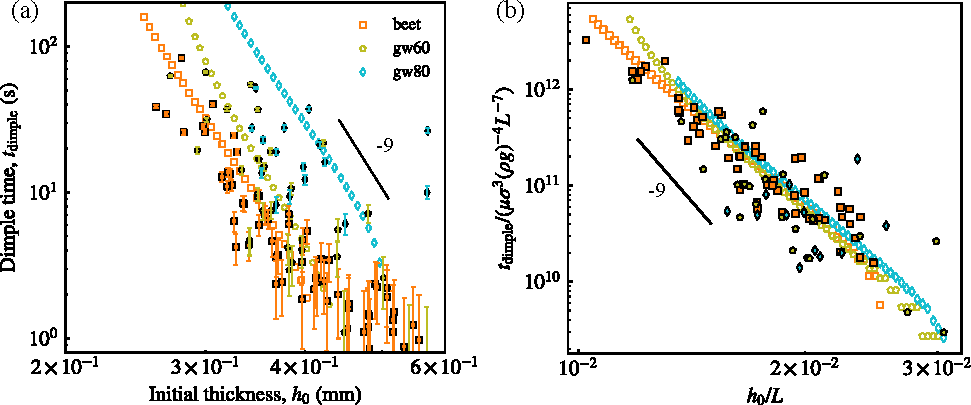
\includegraphics[width=0.8\linewidth]{good_collapse}
    \caption{Compare $t_\mathrm{dimple}$ and non-dimensional $t_\mathrm{dimple}/{\mu \sigma^3 (\rho g)^{-4} L^{-7}}$. (a) Dimple time vs initial thickness. (b) Non-dimensional dimple time vs non-dimensional initial thickness a power-law scaling with an exponent of –9. }
    \label{fig:good_collapse}
\end{figure}

Regarding the error of the measurement, the confocal displacement sensor can measure height at a precision of $\pm 2\;\mathrm{\mu m}$ . According to the equipment precision, we estimate the error of the height ratio to be 0.01. This error is smaller than the marker size of the height ratio vs. time plot (Fig.~5c).

The error associated with the dimple time can be estimated as the scanning frequency. Since it takes about 1 second to scan the surface, the error of dimple time would be on the order of 1 second. To provide readers with an idea of the error associated with our measurement, we added error bars in Figs.~5(c) and 5(d) to indicate the experimental error. We also added a description of the errorbar in the caption.

\hl{
The errorbars indicate the error associated with the precision of the height measurement, which is estimated to be $\pm 0.01$. … The errorbars indicate the error associated with the surface scan process, which is estimated to be $\pm 1$ second.
}

\bigskip
\begin{siderules}
\textbf{Comment 5:} \textit{Finally, does the size of the beet slice (thickness and radius) matter at all in dimple formation? Or are they irrelevant as long as they are much smaller than the container size. I would like a bit more details about the potential effects of the solid geometry on the observed phenomenon.}
\end{siderules}

\textbf{Response:} The radius of the beet slice does not matter as long as it is much bigger than the capillary length. The thickness also does not matter, unless it is much thinner than the stationary contact line height (a few mm, the capillary length $\lambda=\sqrt{\sigma/\rho g}$). 
In the case of a very thin slice, the radius might start to matter, since the suction flow would rely on the wetting of the top surface, instead of the side.

The container size could matter, if it limits the length of the thin film. 
As we showed in the answer to the previous question, when the film is very short, the length of the film becomes a very relevant factor for the dimple time. 

Our study suggests that solid geometries do not influence the dimple formation / dimple time much, as long as it is large enough to induce a sufficient rise of the contact line. 
The only exception is that if the solid is much shorter than $\lambda$, the suction flow might not be sufficient to form a deep dimple. 


\end{document}
